\documentclass{beamer}

\usepackage[utf8]{inputenc}
\usepackage{amsmath,amsfonts,amssymb}
\usepackage{graphicx}
\usepackage{tikz}
\usepackage{listings}
\usepackage{booktabs}
\usetikzlibrary{arrows.meta,positioning}
\graphicspath{{../}}

% KCPC clean theme: Year 1 Week 3 and Year 2 Pair 01 W1.
\usetheme{default}
\useinnertheme{rectangles}
\useoutertheme{default}
\setbeamertemplate{navigation symbols}{}
\definecolor{kcpc-bg}{RGB}{250,250,250}
\definecolor{kcpc-text}{RGB}{20,20,20}
\definecolor{kcpc-muted}{RGB}{90,90,90}
\definecolor{kcpc-red}{RGB}{176,0,0}
\setbeamercolor{background canvas}{bg=kcpc-bg}
\setbeamercolor{normal text}{fg=kcpc-text}
\setbeamercolor{frametitle}{fg=kcpc-text,bg=kcpc-bg}
\setbeamercolor{title}{fg=kcpc-text}
\setbeamercolor{subtitle}{fg=kcpc-muted}
\setbeamercolor{structure}{fg=kcpc-red}
\setbeamercolor{alerted text}{fg=kcpc-red}
\setbeamerfont{title}{series=\bfseries,size=\Large}
\setbeamerfont{frametitle}{series=\bfseries,size=\large}
\setlength{\parskip}{0.4em}
\setbeamertemplate{itemize item}{$\rightarrow$}
\setbeamertemplate{itemize subitem}{$\rightarrow$}
\setbeamertemplate{headline}{%
  \vspace{0.2cm}\hspace{0.2cm}%
  \textcolor{kcpc-muted}{\small\insertsection}\hfill
}
\setbeamertemplate{footline}{%
  \hspace{0.2cm}\textcolor{kcpc-muted}{\small KCPC}\hfill
  \textcolor{kcpc-muted}{\small\insertframenumber}\hspace{0.3cm}\vspace{0.3cm}
}
\setbeamertemplate{background}{%
  \begin{tikzpicture}[remember picture,overlay]
    \node[opacity=0.035,at=(current page.center)]
      {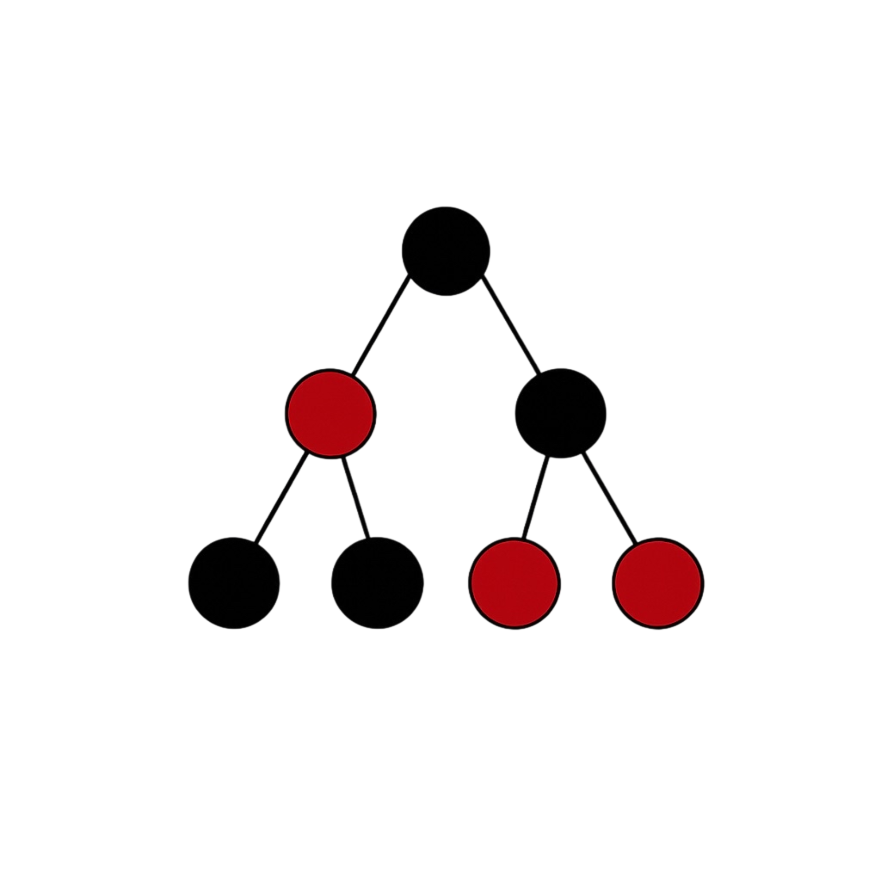
\includegraphics[width=0.55\paperwidth]{kcpc-logo.png}};
  \end{tikzpicture}%
}
\hypersetup{colorlinks=true,linkcolor=kcpc-red,urlcolor=kcpc-red}
\renewcommand{\appendixname}{Appendix}
\lstset{
  language=Python,
  basicstyle=\ttfamily\footnotesize,
  keywordstyle=\color{kcpc-red},
  commentstyle=\color{kcpc-muted},
  stringstyle=\color{kcpc-muted},
  showstringspaces=false,
  columns=fullflexible,
  keepspaces=true,
  aboveskip=0.3em,
  belowskip=0.3em
}
\tikzset{
  vertex/.style={circle,draw=kcpc-text,fill=kcpc-bg,
    minimum size=7mm,inner sep=1pt,font=\small},
  source/.style={vertex,draw=kcpc-red,very thick},
  edge/.style={thick},
  directed/.style={edge,-{Stealth[length=2mm]}},
  weight/.style={fill=kcpc-bg,inner sep=1.5pt,font=\small}
}

% Every edge is drawn here once; the walkthrough treats these as undirected.
\newcommand{\dijkstragraph}{%
  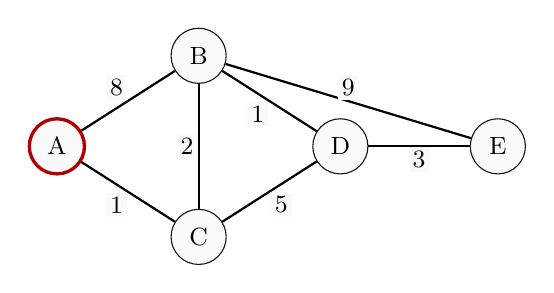
\begin{tikzpicture}[x=1cm,y=1cm]
    \node[source] (A) at (0,0) {A};
    \node[vertex] (B) at (1.8,1.15) {B};
    \node[vertex] (C) at (1.8,-1.15) {C};
    \node[vertex] (D) at (3.6,0) {D};
    \node[vertex] (E) at (5.6,0) {E};
    \draw[edge] (A) -- node[weight,above left] {8} (B);
    \draw[edge] (A) -- node[weight,below left] {1} (C);
    \draw[edge] (B) -- node[weight,left] {2} (C);
    \draw[edge] (B) -- node[weight,below left] {1} (D);
    \draw[edge] (C) -- node[weight,below right] {5} (D);
    \draw[edge] (B) -- node[weight,above] {9} (E);
    \draw[edge] (D) -- node[weight,below] {3} (E);
  \end{tikzpicture}%
}
\newcommand{\binarygraph}{%
  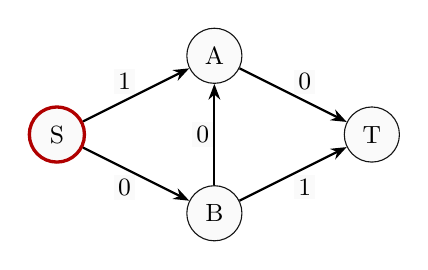
\begin{tikzpicture}[x=1cm,y=1cm]
    \node[source] (S) at (0,0) {S};
    \node[vertex] (A) at (2,1) {A};
    \node[vertex] (B) at (2,-1) {B};
    \node[vertex] (T) at (4,0) {T};
    \draw[directed] (S) -- node[weight,above left] {1} (A);
    \draw[directed] (S) -- node[weight,below left] {0} (B);
    \draw[directed] (B) -- node[weight,left] {0} (A);
    \draw[directed] (A) -- node[weight,above right] {0} (T);
    \draw[directed] (B) -- node[weight,below right] {1} (T);
  \end{tikzpicture}%
}
\newcommand{\arrowgrid}{%
  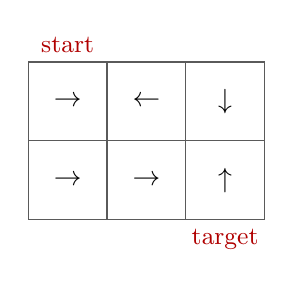
\begin{tikzpicture}[x=1cm,y=1cm]
    \foreach \r in {0,1} {
      \foreach \c in {0,1,2} {
        \draw[kcpc-muted] (\c,-\r) rectangle ++(1,-1);
      }
    }
    \node at (0.5,-0.5) {$\rightarrow$};
    \node at (1.5,-0.5) {$\leftarrow$};
    \node at (2.5,-0.5) {$\downarrow$};
    \node at (0.5,-1.5) {$\rightarrow$};
    \node at (1.5,-1.5) {$\rightarrow$};
    \node at (2.5,-1.5) {$\uparrow$};
    \node[kcpc-red,above,font=\small] at (0.5,0) {start};
    \node[kcpc-red,below,font=\small] at (2.5,-2) {target};
  \end{tikzpicture}%
}

\title{Graphs II}
\subtitle{Distance, Constraints, and Logical Structure\\Dijkstra and 0--1 BFS}
\author{KCPC}
\institute{In collaboration with KCL Tech\\2025--2026 partnership}
% The original source used today's date, not a recorded workshop date.
\date{Week 5}

\begin{document}

\begin{frame}[plain]
  \titlepage
\end{frame}

\begin{frame}{Today's route}
  \begin{enumerate}
    \item Model a graph; recall DFS, BFS and multi-source BFS.
    \item Find minimum total cost with \textbf{Dijkstra}.
    \item Specialise to binary costs with \textbf{0--1 BFS}.
    \item Translate grids and path variants into the right model.
  \end{enumerate}
  \medskip
  Live examples: problems \textbf{1--3}. Then try the core set.

  Checkpoints \textbf{C1--C6} have full answers \emph{after the conclusion}.
\end{frame}

\section{Graph foundations}

\begin{frame}{A graph is a set of states and moves}
  \begin{columns}[c]
    \begin{column}{0.42\textwidth}
      \centering
      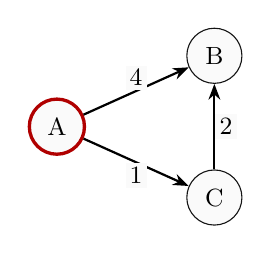
\begin{tikzpicture}
        \node[source] (A) at (0,0) {A};
        \node[vertex] (B) at (2,0.9) {B};
        \node[vertex] (C) at (2,-0.9) {C};
        \draw[directed] (A) -- node[weight,above] {4} (B);
        \draw[directed] (A) -- node[weight,below] {1} (C);
        \draw[directed] (C) -- node[weight,right] {2} (B);
      \end{tikzpicture}
    \end{column}
    \begin{column}{0.55\textwidth}
      \begin{itemize}
        \item \textbf{Vertex}: a state, such as a city or grid cell.
        \item \textbf{Edge}: a legal move between states.
        \item \textbf{Weight}: the cost of that move.
        \item Arrows mean \textbf{directed}: the reverse move is not automatic.
      \end{itemize}
    \end{column}
  \end{columns}
  \medskip
  A path follows edges. Its usual cost is the \textbf{sum of edge weights}.
\end{frame}

\begin{frame}[fragile]{Store neighbours in an adjacency list}
  For the previous directed graph:
\begin{lstlisting}
adj = {
    "A": [("B", 4), ("C", 1)],
    "B": [],
    "C": [("B", 2)]
}
\end{lstlisting}
  \begin{itemize}
    \item \texttt{adj[u]} contains pairs \texttt{(neighbour, weight)}.
    \item For an \textbf{undirected} edge, insert \emph{both} directions.
    \item Usually number vertices $0,\ldots,V-1$ and use a list of lists.
    \item $V$ vertices and $E$ edges take $O(V+E)$ storage.
  \end{itemize}
\end{frame}

\begin{frame}{DFS reaches; BFS finds fewest edges}
  \begin{itemize}
    \item \textbf{DFS}: follow a branch, then backtrack using a stack.\newline
      Good for reachability; the first path found need not be shortest.
    \item \textbf{BFS}: use a FIFO (first in, first out) queue, visiting one layer at a time.\newline
      A vertex first reached from layer $k$ has distance $k+1$.
    \item In ordinary BFS, mark a vertex when \textbf{enqueuing} it.\newline
      This avoids repeatedly adding the same vertex.
  \end{itemize}
  \medskip
  BFS minimises \textbf{edge count}: also minimum cost when every edge
  has the same positive cost. Both traversals take $O(V+E)$ time.
\end{frame}

\begin{frame}{Multi-source BFS: nearest of many starts}
  \textbf{Problem 7: LC542, 01 Matrix.} Distance to the nearest zero.
  \[
    \begin{pmatrix}0&1&1\\1&1&1\\1&1&0\end{pmatrix}
    \quad\longrightarrow\quad
    \begin{pmatrix}0&1&2\\1&2&1\\2&1&0\end{pmatrix}
  \]
  \begin{enumerate}
    \item Set every zero's distance to $0$ and put \textbf{all zeros} in one queue.
    \item Other cells start at $\infty$; expand four-direction neighbours.
    \item On first discovery, set $\mathrm{dist}[v]=\mathrm{dist}[u]+1$.
  \end{enumerate}
  The first wave to reach a cell comes from its nearest source.
  One BFS, $O(RC)$ time; no separate search for each zero.
\end{frame}

\begin{frame}{Try yourself C1: nearest zero}
  \[
    \begin{pmatrix}1&1&0\\1&1&1\\0&1&1\end{pmatrix}
  \]
  You may move up, down, left or right within the grid.
  \begin{enumerate}
    \item Which cells enter the queue initially, and at what distance?
    \item Compute the complete distance matrix.
    \item Why would a DFS's first-found route not justify these distances?
  \end{enumerate}
  \medskip
  Coordinates in this deck are \textbf{zero-based}: top left is $(0,0)$.
\end{frame}

\section{Dijkstra: nonnegative edge costs}

\begin{frame}{Fewest edges can be expensive}
  \centering
  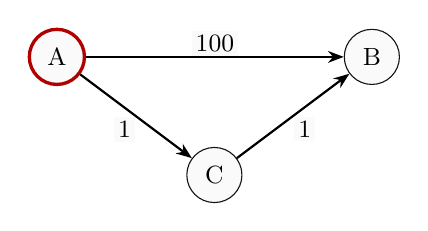
\begin{tikzpicture}
    \node[source] (A) at (0,0) {A};
    \node[vertex] (B) at (4,0) {B};
    \node[vertex] (C) at (2,-1.5) {C};
    \draw[directed] (A) -- node[weight,above] {100} (B);
    \draw[directed] (A) -- node[weight,below left] {1} (C);
    \draw[directed] (C) -- node[weight,below right] {1} (B);
  \end{tikzpicture}
  \[
    A\to B:\ 100
    \qquad\qquad
    A\to C\to B:\ 1+1=2
  \]
  \raggedright
  Ordinary BFS prefers one edge. We need to prefer \textbf{lower total cost}.

  Dijkstra handles \textbf{nonnegative weights}, including zero.
\end{frame}

\begin{frame}{Relaxation: improve a best-known route}
  \begin{itemize}
    \item $\mathrm{dist}[v]$ is the cheapest route \textbf{found so far} to $v$.
    \item Initially $\mathrm{dist}[s]=0$; everything else is $\infty$.
    \item From $u$, try each edge $u\to v$ with weight $w$:
  \end{itemize}
  \[
    \mathrm{candidate}=\mathrm{dist}[u]+w.
  \]
  If $\mathrm{candidate}<\mathrm{dist}[v]$, replace the label and queue it.
  This improvement is called \textbf{relaxing} the edge.

  \textbf{Which queued route next?} Use a \textbf{min-heap}: it removes the
  entry with the smallest distance, not the oldest entry.
\end{frame}

\begin{frame}{The invariant that makes Dijkstra safe}
  \textbf{Invariant:} when a \emph{current} minimum-distance entry for $u$
  is removed, its distance is the true shortest distance.
  \begin{itemize}
    \item Why? A cheaper route would have to pass through an unprocessed
      vertex with a smaller distance first.
    \item That vertex would have been processed earlier. Nonnegative
      edges cannot make a later route suddenly cheaper.
    \item Hence $u$ is \textbf{settled}: its label will not improve again.
  \end{itemize}
  \medskip
  A negative edge breaks this argument. Do \textbf{not} use Dijkstra
  for general negative-weight graphs.
\end{frame}

\begin{frame}[fragile]{Dijkstra in Python: lazy min-heap}
  Here \texttt{adj[u]} is a list of \texttt{(v, w)} pairs; vertices are integers.
\begin{lstlisting}
from heapq import heappop, heappush

def dijkstra(adj, src):
    dist = [float("inf")] * len(adj)
    dist[src] = 0
    heap = [(0, src)]
    while heap:
        d, u = heappop(heap)
        if d != dist[u]:
            continue
        for v, w in adj[u]:
            nd = d + w
            if nd < dist[v]:
                dist[v] = nd
                heappush(heap, (nd, v))
    return dist
\end{lstlisting}
\end{frame}

\begin{frame}{Stale entries and the right time to stop}
  \begin{itemize}
    \item Heap entries are \textbf{snapshots} \texttt{(distance, vertex)}.
      Improving a label adds a new entry; the old one stays in the heap.
    \item If popped $d\ne\mathrm{dist}[u]$, the snapshot is \textbf{stale}.
      Skip it without scanning neighbours.
    \item \textbf{One target?} After the stale check, stop when the target
      is \emph{popped}. Its distance is now final.
    \item \textbf{All distances?} Keep going until the heap is empty.
  \end{itemize}
  \medskip
  \alert{Do not stop on first discovery or mark a vertex final on insertion.}
\end{frame}

\begin{frame}[fragile]{Live 1 / problem 1: GFG Dijkstra}
  \href{https://www.geeksforgeeks.org/problems/implementing-dijkstra-set-1-adjacency-matrix/1}{\textbf{GFG: Dijkstra Algorithm}}
  currently supplies an \textbf{undirected edge list}, not a matrix.
\begin{lstlisting}
class Solution:
    def dijkstra(self, V, edges, src):
        adj = [[] for _ in range(V)]
        for u, v, w in edges:
            adj[u].append((v, w))
            adj[v].append((u, w))
        return dijkstra(adj, src)
\end{lstlisting}
  This wrapper calls the previous helper. Return distances in vertex order.

  The historical URL still says \texttt{adjacency-matrix}; use the
  \textbf{current platform signature} \texttt{V, edges, src}.
\end{frame}

\begin{frame}{Live 1: a graph we can trace exactly}
  \centering
  \dijkstragraph
  \par\medskip
  \raggedright
  \textbf{Undirected.} Source A; target E. Labels A--E map to integers 0--4.
  \[
    \begin{aligned}
      \mathrm{edges}=[&(0,1,8),(0,2,1),(1,2,2),(1,3,1),\\
                      &(2,3,5),(1,4,9),(3,4,3)].
    \end{aligned}
  \]
  Predict the order of \textbf{valid pops}. An edge's weight is not
  necessarily the distance of its endpoint.
\end{frame}

\begin{frame}{Live 1: reproducible heap trace}
  \small
  Entries below are \textbf{(distance, vertex)}, displayed in sorted order.\newline
  A binary heap need not store them in this visual order internally.
  \medskip
  \centering
  \begin{tabular}{@{}lll@{}}
    \toprule
    Pop & Improved labels & Pending entries after the pop \\
    \midrule
    $(0,\mathrm A)$ & B: 8, C: 1 & $(1,\mathrm C),(8,\mathrm B)$ \\
    $(1,\mathrm C)$ & B: 3, D: 6 & $(3,\mathrm B),(6,\mathrm D),(8,\mathrm B)$ \\
    $(3,\mathrm B)$ & D: 4, E: 12 & $(4,\mathrm D),(6,\mathrm D),(8,\mathrm B),(12,\mathrm E)$ \\
    $(4,\mathrm D)$ & E: 7 & $(6,\mathrm D),(7,\mathrm E),(8,\mathrm B),(12,\mathrm E)$ \\
    $(6,\mathrm D)$ & stale: skip & $(7,\mathrm E),(8,\mathrm B),(12,\mathrm E)$ \\
    $(7,\mathrm E)$ & none & $(8,\mathrm B),(12,\mathrm E)$ \\
    $(8,\mathrm B)$ & stale: skip & $(12,\mathrm E)$ \\
    $(12,\mathrm E)$ & stale: skip & empty \\
    \bottomrule
  \end{tabular}
  \par\medskip
  \raggedright
  Final distances: $[0,3,1,4,7]$. Shortest route to E:
  $\mathrm A\to\mathrm C\to\mathrm B\to\mathrm D\to\mathrm E$.

  For E only, stop at \textbf{(7, E)}, not when E is first labelled 12.
\end{frame}

\begin{frame}{Try yourself C2: a free final edge}
  \centering
  \dijkstragraph
  \par\medskip
  \raggedright
  Change \textbf{only D--E from weight 3 to weight 0}.
  \begin{enumerate}
    \item Find the new final distances from A and a shortest route to E.
    \item When is E first discovered? When is it safe to stop?
    \item List the valid pops, breaking equal-distance ties alphabetically.
  \end{enumerate}
\end{frame}

\begin{frame}{Live 2 / problem 2: Network Delay Time}
  \textbf{LC743:} a signal starts at vertex $k$. When has \emph{every} vertex
  received it? Edges are \textbf{directed} travel times.
  \begin{columns}[c]
    \begin{column}{0.45\textwidth}
      \centering
      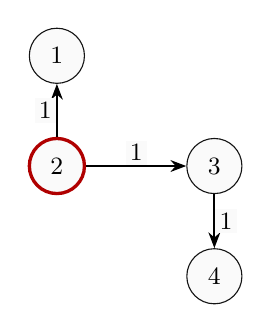
\begin{tikzpicture}
        \node[source] (two) at (0,0) {2};
        \node[vertex] (one) at (0,1.4) {1};
        \node[vertex] (three) at (2,0) {3};
        \node[vertex] (four) at (2,-1.4) {4};
        \draw[directed] (two) -- node[weight,left] {1} (one);
        \draw[directed] (two) -- node[weight,above] {1} (three);
        \draw[directed] (three) -- node[weight,right] {1} (four);
      \end{tikzpicture}
    \end{column}
    \begin{column}{0.52\textwidth}
      $n=4,\ k=2$.\newline
      Input: $(2,1,1)$, $(2,3,1)$, $(3,4,1)$.

      Distances in order 1--4:\newline
      $[1,0,1,2]$.

      Return $\max_v\mathrm{dist}[v]=\boxed{2}$.
    \end{column}
  \end{columns}
  If any vertex is unreachable, return $-1$.
  With a size $n+1$ array, ignore unused index 0 in the answer.
\end{frame}

\begin{frame}{Dijkstra: implementation checklist}
  \begin{itemize}
    \item All weights must be \textbf{nonnegative}; zero-cost edges are fine.
    \item Relax only on a \textbf{strict improvement}; stale pops do no work.
    \item Unreachable vertices stay at $\infty$. Use sufficiently wide
      integers in C++ for sums of many weights.
    \item To recover a route, set \texttt{parent[v] = u} on improvement;
      follow parents backwards from the target.
  \end{itemize}
  \medskip
  \small
  Lazy heap: $O(V+E\log(E+1))$ time, $O(V+E)$ space.
  For a simple graph, the usual time bound is $O((V+E)\log V)$.
\end{frame}

\section{0--1 BFS: two distance levels}

\begin{frame}{Binary costs do not need a full heap}
  Suppose every edge weight is \textbf{0 or 1}.
  \begin{itemize}
    \item From a route of cost $d$, the next cost is only $d$ or $d+1$.
    \item A \textbf{deque} lets us insert at either end and pop from the front.
    \item A weight-0 improvement goes to the \textbf{front}: same cost layer.
    \item A weight-1 improvement goes to the \textbf{back}: next cost layer.
  \end{itemize}
  \medskip
  This is \textbf{0--1 BFS}: Dijkstra's ordering, without a heap.
  Ordinary FIFO BFS would count edges, not total cost.
\end{frame}

\begin{frame}{The deque invariant: compare stored keys}
  \textbf{Store snapshots $(d,u)$}, just as in the heap.
  \[
    \underbrace{d,\ d,\ d}_{\text{front level}}
    \quad
    \underbrace{d+1,\ d+1}_{\text{next level}}
  \]
  \begin{itemize}
    \item Stored distance keys are nondecreasing, with at most
      \textbf{two adjacent levels}.
    \item On a current pop of cost $d$, front-inserting $d$ or
      back-inserting $d+1$ preserves this order.
    \item Labels may improve while old snapshots remain. Skip a pop
      when $d\ne\mathrm{dist}[u]$.
  \end{itemize}
  The current front is minimum, so the same settling argument applies.
  Do not confuse \emph{stored keys} with changing \texttt{dist} labels.
\end{frame}

\begin{frame}[fragile]{0--1 BFS in Python}
\begin{lstlisting}
from collections import deque

def zero_one_bfs(adj, src):
    dist = [float("inf")] * len(adj)
    dist[src] = 0
    q = deque([(0, src)])
    while q:
        d, u = q.popleft()
        if d != dist[u]:
            continue
        for v, w in adj[u]:
            nd = d + w
            if nd < dist[v]:
                dist[v] = nd
                if w == 0:
                    q.appendleft((nd, v))
                else:
                    q.append((nd, v))
    return dist
\end{lstlisting}
\end{frame}

\begin{frame}{Live: a zero-cost detour beats discovery}
  \centering
  \binarygraph
  \par\medskip
  \raggedright
  \textbf{Directed.} Scan outgoing edges in exactly this order:
  \[
    \begin{aligned}
      S &: [(A,1),(B,0)] & A &: [(T,0)]\\
      B &: [(A,0),(T,1)] & T &: []
    \end{aligned}
  \]
  A is first discovered at 1, but $S\to B\to A$ costs 0.
  Predict what happens to the \emph{old} entry for A.
\end{frame}

\begin{frame}{Live: exact deque trace, front on the left}
  \small
  Start with $[(0,S)]$. Each entry is a stored \textbf{(distance, vertex)}.
  \medskip
  \centering
  \begin{tabular}{@{}lll@{}}
    \toprule
    Pop & Improved labels & Deque after the pop \\
    \midrule
    $(0,S)$ & A: 1, B: 0 & $[(0,B),(1,A)]$ \\
    $(0,B)$ & A: 0, T: 1 & $[(0,A),(1,A),(1,T)]$ \\
    $(0,A)$ & T: 0 & $[(0,T),(1,A),(1,T)]$ \\
    $(0,T)$ & none & $[(1,A),(1,T)]$ \\
    $(1,A)$ & stale: skip & $[(1,T)]$ \\
    $(1,T)$ & stale: skip & empty \\
    \bottomrule
  \end{tabular}
  \par\medskip
  \raggedright
  All four final distances are 0.
  A shortest route to T is $S\to B\to A\to T$.

  We could stop at the \textbf{current} pop $(0,T)$, after the stale check.
\end{frame}

\begin{frame}{Try yourself C3: two tempting mistakes}
  Use the previous directed graph and the same edge-scan order.
  \begin{enumerate}
    \item Suppose we mark a vertex visited \emph{when enqueuing}, and
      never allow it to improve. What wrong distance reaches T?
    \item Keep the correct distance updates, but change the stale test
      to always process old entries. What work is unnecessarily repeated?
    \item Why must the relaxation test use $<$, not $\leq$, if a
      zero-cost cycle exists?
  \end{enumerate}
  \medskip
  Explain the role of \textbf{distance improvements}, not just queue order.
\end{frame}

\begin{frame}{0--1 BFS: what the guarantee depends on}
  \begin{itemize}
    \item Weights really must lie in $\{0,1\}$, not just be integers.
    \item Never make first \emph{discovery} final. A zero-cost detour may
      improve an already queued vertex.
    \item A current pop is settled; stale snapshots do not rescan edges.
    \item Strict improvements also prevent endless requeuing around
      zero-cost cycles.
  \end{itemize}
  \medskip
  $O(V+E)$ time: each vertex's outgoing edges are scanned once on its
  current pop; each successful relaxation adds one snapshot.

  $O(V+E)$ space including adjacency lists and queued snapshots.
\end{frame}

\section{Modelling and problem selection}

\begin{frame}{A grid is an implicit graph}
  \begin{itemize}
    \item \textbf{State}: a cell $(r,c)$; \textbf{edge}: one legal move.
    \item Generate neighbours when needed: usually
      $(r\pm1,c)$ and $(r,c\pm1)$.
    \item Reject out-of-bounds cells and any forbidden destinations.
    \item Define the \textbf{cost of the move}, then select the algorithm.
  \end{itemize}
  \medskip
  No need to build an adjacency list for every cell.
  An $R\times C$ four-neighbour grid has $RC$ vertices and $O(RC)$ edges.

  A rectangular drawing does \emph{not} imply unweighted BFS.
\end{frame}

\begin{frame}{Live 3 / problem 3: arrow-grid costs}
  \textbf{LC1368:} change as few cell arrows as possible to obtain a path
  from top left to bottom right.
  \begin{columns}[c]
    \begin{column}{0.38\textwidth}
      \centering
      \arrowgrid
    \end{column}
    \begin{column}{0.59\textwidth}
      Every in-bounds orthogonal move is allowed.
      \[
        w(u,v)=
        \begin{cases}
          0 & \text{follow the arrow at }u,\\
          1 & \text{otherwise.}
        \end{cases}
      \]
      The arrow belongs to the cell we \textbf{leave}, not the one we enter.
    \end{column}
  \end{columns}
  \medskip
  Platform encoding: $1=\rightarrow$, $2=\leftarrow$,
  $3=\downarrow$, $4=\uparrow$. Use \textbf{0--1 BFS}.
\end{frame}

\begin{frame}{Try yourself C4 / live 3: escape the arrow loop}
  \begin{columns}[c]
    \begin{column}{0.38\textwidth}
      \centering
      \arrowgrid
    \end{column}
    \begin{column}{0.59\textwidth}
      Input:
      $\begin{pmatrix}1&2&3\\1&1&4\end{pmatrix}$.
      \begin{enumerate}
        \item What cells can we reach at cost 0 from $(0,0)$?
        \item Find a minimum-cost route to $(1,2)$.
        \item Give a lower bound proving that your route is optimal.
      \end{enumerate}
    \end{column}
  \end{columns}
  \medskip
  Following arrows forever can loop. A shortest route can be chosen
  without cycles, so paying for a departure corresponds to changing
  that cell's arrow once.
\end{frame}

\begin{frame}{Sometimes the cost belongs to the destination}
  \textbf{Problem 6: LC2290, obstacle removal.}
  \[
    w\bigl((r,c),(r',c')\bigr)=\mathrm{grid}[r'][c']\in\{0,1\}.
  \]
  \begin{itemize}
    \item Entering an obstacle costs 1; entering an empty cell costs 0.
      Use \textbf{0--1 BFS}. The source is empty, so start at cost 0.
    \item Do not charge the cell being left. This differs from LC1368.
  \end{itemize}
  \medskip
  \textbf{Problems 9--11: Euler matrix path sums.}
  \begin{itemize}
    \item Entering $v$ costs $\mathrm{matrix}[v]$.
    \item The initial cell is counted too:
      $\mathrm{dist}[s]=\mathrm{matrix}[s]$, not 0.
  \end{itemize}
\end{frame}

\begin{frame}{Movement rules change the graph}
  \textbf{Problems 9--11: positive matrix entries; destination-entry costs.}
  \medskip
  \small
  \setlength{\tabcolsep}{4pt}
  \begin{tabular}{@{}llll@{}}
    \toprule
    Problem & Moves & Start / finish & Method \\
    \midrule
    9: Euler 81 & right, down & top left / bottom right & DP or Dijkstra \\
    10: Euler 82 & up, down, right & any left / any right & Dijkstra \\
    11: Euler 83 & four directions & top left / bottom right & Dijkstra \\
    \bottomrule
  \end{tabular}
  \normalsize
  \medskip
  For Euler 82, seed the heap with \textbf{every left-column cell},
  each at its own entry value. Answer: minimum distance in the right column.

  For Euler 81, right/down moves let a simple row-by-row DP compute
  each cell from its upper and left neighbours.
\end{frame}

\begin{frame}{Problem 8: Wizard in Maze}
  \textbf{ABC176D} has two kinds of moves:
  \begin{itemize}
    \item Walk to an orthogonally adjacent \textbf{open} cell: cost 0.
    \item Warp to an \textbf{open} cell within a $5\times5$ square
      centred on the current cell: cost 1.
    \item For a warp, both row and column offsets may be at most 2
      in absolute value. Intermediate walls do not matter.
  \end{itemize}
  \medskip
  Minimise the number of warps with \textbf{0--1 BFS}, not the number of steps.

  Check the landing cell. A warp does \emph{not} allow landing on a wall.
\end{frame}

\begin{frame}{Problem 4: maximise a product, not minimise a sum}
  \textbf{LC1514: Path with Maximum Probability.}
  \[
    P(s\leadsto t)=\prod_{e\text{ on the path}}p_e,
    \qquad 0\leq p_e\leq1.
  \]
  \begin{itemize}
    \item Start with $\mathrm{best}[s]=1$; other probabilities are 0.
    \item Candidate through $u$: $\mathrm{best}[u]\cdot p(u,v)$.
      Update when this is \textbf{larger}.
    \item Use a \textbf{max-heap}; Python's min-heap can store negative
      probabilities. Skip stale snapshots as before.
  \end{itemize}
  Extending a route cannot increase its probability. Therefore the
  current \emph{maximum} pop is final; the target may be returned then.
  Return 0 if no route exists.
\end{frame}

\begin{frame}{Problem 5: minimise the largest step}
  \textbf{LC1631: Path with Minimum Effort.}
  \[
    \mathrm{effort}(P)=\max_{(u,v)\text{ on }P}|h[u]-h[v]|.
  \]
  \begin{itemize}
    \item Start at effort 0. This is not a sum of height differences.
    \item Relax with
      $\mathrm{candidate}=\max(\mathrm{effort}[u],|h[u]-h[v]|)$.
    \item Keep smaller candidates and use a \textbf{min-heap}.
  \end{itemize}
  Extending a route cannot reduce its largest step. The same
  current-minimum settling rule applies.

  \textbf{Pattern:} define how a path score extends, then justify why
  the best current pop cannot improve later.
\end{frame}

\begin{frame}{Try yourself C5: what are we optimising?}
  These are three \textbf{separate} mini-problems.
  \begin{enumerate}
    \item Euler 81 rules on
      $\begin{pmatrix}2&8\\1&3\end{pmatrix}$:
      find the minimum path sum, including the starting cell.
    \item A direct route has success probability $0.75$.
      A two-edge route has probabilities $0.8$ and $0.9$.
      Which route is better?
    \item Route A has step differences $2,9$; route B has $6,6$.
      Which has smaller \emph{effort}?
  \end{enumerate}
  For each, state the operation used to extend a path score.
\end{frame}

\begin{frame}{A constraint may require a bigger state}
  \textbf{Problem 12: LC1928, minimum fee within a time limit.}

  At the same city $u$, we might arrive:
  \begin{itemize}
    \item cheaply but slowly: fee 3, time used 9;
    \item expensively but quickly: fee 6, time used 3.
  \end{itemize}
  Neither arrival is automatically better: future feasibility depends
  on the \textbf{time remaining}.

  Keep a state such as $(\mathrm{city},\mathrm{timeUsed})$, with the
  best fee for each state. One \texttt{dist[city]} can discard a necessary route.

  The source fee is counted; travelling adds time and the destination's fee.
\end{frame}

\begin{frame}{Try yourself C6: keep the useful arrival}
  Continue the previous example:
  \begin{itemize}
    \item Total time limit: 10.
    \item The only move from $u$ to the target takes 3 more time units.
    \item The target's entry fee is 2.
  \end{itemize}
  \begin{enumerate}
    \item Which arrival at $u$ can finish? What is its total fee?
    \item Why does retaining only the cheapest fee at $u$ fail?
    \item How would you label the states and reject illegal transitions?
  \end{enumerate}
\end{frame}

\begin{frame}{Choose by the model, not the problem's title}
  \small
  \begin{tabular}{@{}lll@{}}
    \toprule
    Need / edge costs & First choice & Time \\
    \midrule
    Reachability only & DFS or BFS & $O(V+E)$ \\
    Unit / equal positive cost & BFS & $O(V+E)$ \\
    Costs 0 or 1 & 0--1 BFS & $O(V+E)$ \\
    General nonnegative costs & Dijkstra & heap logarithm \\
    General negative costs & e.g. Bellman--Ford & outside today's scope \\
    \bottomrule
  \end{tabular}
  \normalsize
  \medskip
  Multiple starts? Seed \textbf{all sources} at their correct initial scores.

  Time, fuel, keys or remaining moves affect future choices?
  They may belong in the \textbf{state}, not just in an edge weight.
\end{frame}

\begin{frame}{Problem sheet: live examples 1--3}
  \begin{enumerate}
    \item \href{https://www.geeksforgeeks.org/problems/implementing-dijkstra-set-1-adjacency-matrix/1}{\textbf{GFG: Dijkstra Algorithm}}\\
      Undirected edge list; return every distance.
    \item \href{https://leetcode.com/problems/network-delay-time/}{\textbf{LC743: Network Delay Time}}\\
      Directed edges; return the maximum distance, or $-1$.
    \item \href{https://leetcode.com/problems/minimum-cost-to-make-at-least-one-valid-path-in-a-grid/}{\textbf{LC1368: Minimum Cost to Make at Least}}\\
      \href{https://leetcode.com/problems/minimum-cost-to-make-at-least-one-valid-path-in-a-grid/}{\textbf{One Valid Path in a Grid}}\\
      Arrow-departure costs; 0--1 BFS.
  \end{enumerate}
  \medskip
  Use the worked traces to explain each improvement, not just the final answer.
\end{frame}

\begin{frame}{Problem sheet: core practice 4--11}
  \small
  \begin{tabular}{@{}rll@{}}
    \toprule
    No. & Problem & Modelling cue \\
    \midrule
    4 & \href{https://leetcode.com/problems/path-with-maximum-probability/}{LC1514: Maximum Probability} & product; max-heap \\
    5 & \href{https://leetcode.com/problems/path-with-minimum-effort/}{LC1631: Minimum Effort} & largest step; min-heap \\
    6 & \href{https://leetcode.com/problems/minimum-obstacle-removal-to-reach-corner/}{LC2290: Obstacle Removal} & destination-entry 0/1 cost \\
    7 & \href{https://leetcode.com/problems/01-matrix/}{LC542: 01 Matrix} & multi-source \emph{ordinary} BFS \\
    8 & \href{https://atcoder.jp/contests/abc176/tasks/abc176_d}{ABC176D: Wizard in Maze} & free steps, paid warps \\
    9 & \href{https://projecteuler.net/problem=81}{Euler 81: Path Sum, Two Ways} & right/down; DP also works \\
    10 & \href{https://projecteuler.net/problem=82}{Euler 82: Path Sum, Three Ways} & left column as many starts \\
    11 & \href{https://projecteuler.net/problem=83}{Euler 83: Path Sum, Four Ways} & four-direction Dijkstra \\
    \bottomrule
  \end{tabular}
  \normalsize
  \medskip
  Work individually or in small groups. For each problem, first write
  down \textbf{state, legal moves, move cost and initial score}.
\end{frame}

\begin{frame}{Problem sheet: extended challenges 12--15}
  \setbeamertemplate{enumerate item}[default]
  \begin{enumerate}
    \setcounter{enumi}{11}
    \item \href{https://leetcode.com/problems/minimum-cost-to-reach-destination-in-time/}{\textbf{LC1928: Minimum Cost to Reach Destination in Time}}\\
      State expansion: city alone is not enough.
    \item \href{https://codeforces.com/problemset/problem/786/B}{\textbf{CF786B: Legacy}}\\
      Segment-tree graph construction plus Dijkstra.
    \item \href{https://codeforces.com/problemset/problem/715/B}{\textbf{CF715B: Complete The Graph}}\\
      Construct edge weights to meet a shortest-path target.
    \item \href{https://atcoder.jp/contests/abc213/tasks/abc213_e}{\textbf{ABC213E: Stronger Takahashi}}\\
      Advanced 0--1 movement modelling; read the punch rules carefully.
  \end{enumerate}
  \medskip
  Optional stretch work after the core set; these require additional ideas.
\end{frame}

\section{Conclusion}

\begin{frame}{Take away the ordering, not just the code}
  \begin{itemize}
    \item \textbf{Model first}: state, moves, costs and starting score.
    \item \textbf{Dijkstra}: settle the current minimum from a min-heap.
    \item \textbf{0--1 BFS}: cost 0 to the front, cost 1 to the back.
    \item \textbf{Both}: allow improvements, skip stale entries, and only
      early-exit on a current target pop.
  \end{itemize}
  \medskip
  Ask: \emph{What guarantees that the next state I process is already optimal?}

  \textbf{End of main slides.} Checkpoint answers follow in the appendix.
\end{frame}

\appendix
\section{Appendix: checkpoint answers}

\begin{frame}{Answer C1: one queue, two wavefronts}
  \[
    \begin{pmatrix}1&1&0\\1&1&1\\0&1&1\end{pmatrix}
    \quad\longrightarrow\quad
    \begin{pmatrix}2&1&0\\1&2&1\\0&1&2\end{pmatrix}
  \]
  \begin{itemize}
    \item Seed $(0,2)$ and $(2,0)$ at distance 0 \textbf{before} expanding.
    \item Layer 1: $(0,1),(1,2),(1,0),(2,1)$.
    \item Layer 2: $(0,0),(1,1),(2,2)$.
    \item FIFO processing explores all shorter routes first, so first
      discovery is minimal. DFS does not maintain distance layers and
      can find a longer route before a shorter one.
  \end{itemize}
\end{frame}

\begin{frame}{Answer C2: zero edges are still safe}
  With D--E changed to 0:
  \[
    [\mathrm{dist}[A],\mathrm{dist}[B],\mathrm{dist}[C],
      \mathrm{dist}[D],\mathrm{dist}[E]]=[0,3,1,4,4].
  \]
  \begin{itemize}
    \item Route $A\to C\to B\to D\to E$ costs $1+2+1+0=4$.
    \item E is first discovered from B with cost $3+9=12$.
      This is not final.
    \item Current pops are $(0,A),(1,C),(3,B),(4,D),(4,E)$.
      Equal keys use the alphabetical tie rule stated in the question.
    \item Stop safely at $(4,E)$. If continuing, old snapshots
      $(6,D),(8,B),(12,E)$ are skipped.
  \end{itemize}
\end{frame}

\begin{frame}{Answer C3: discovery is not settlement}
  \begin{enumerate}
    \item With enqueue-time visited flags, S fixes A at 1 and B at 0.
      B cannot improve A, and discovers T at 1. A cannot improve T
      either. The wrong answer is \textbf{1}, instead of 0.
    \item Without the stale check, old $(1,A)$ rescans A's outgoing edge,
      and old $(1,T)$ processes T again. Strict relaxation prevents
      new improvements here, but these scans are unnecessary.
    \item With $\leq$, an edge on a zero-cost cycle can requeue a vertex
      at the \emph{same} distance forever. Strict $<$ queues only genuine
      improvements.
  \end{enumerate}
  The correct shortest route is $S\to B\to A\to T$, total cost 0.
\end{frame}

\begin{frame}{Answer C4: exactly one changed arrow}
  \begin{columns}[c]
    \begin{column}{0.38\textwidth}
      \centering
      \arrowgrid
    \end{column}
    \begin{column}{0.59\textwidth}
      Zero-cost reachable cells are just $(0,0)$ and $(0,1)$:
      their arrows point to each other.

      Any route to the target must leave this set, so it costs
      \textbf{at least 1}.
    \end{column}
  \end{columns}
  \medskip
  Route $(0,0)\to(0,1)\to(0,2)\to(1,2)$ has costs $0,1,0$.
  Change $(0,1)$ from left to right. Total $\boxed{1}$ matches the lower bound.

  Alternatively, change $(0,0)$ to down, then follow the bottom row.
\end{frame}

\begin{frame}{Answer C4: a reproducible grid-deque trace}
  \small
  Name cells $\begin{smallmatrix}A&B&C\\D&E&F\end{smallmatrix}$.
  Scan directions \textbf{right, left, down, up}; ignore out-of-bounds moves.
  Entries are \textbf{(stored cost, cell)}, front on the left.
  \medskip
  \centering
  \begin{tabular}{@{}lll@{}}
    \toprule
    Pop & Improved labels & Deque after the pop \\
    \midrule
    $(0,A)$ & B: 0, D: 1 & $[(0,B),(1,D)]$ \\
    $(0,B)$ & C: 1, E: 1 & $[(1,D),(1,C),(1,E)]$ \\
    $(1,D)$ & none & $[(1,C),(1,E)]$ \\
    $(1,C)$ & F: 1 & $[(1,F),(1,E)]$ \\
    $(1,F)$ & none & $[(1,E)]$ \\
    $(1,E)$ & none & empty \\
    \bottomrule
  \end{tabular}
  \par\medskip
  \raggedright
  Complete distances: $\begin{pmatrix}0&0&1\\1&1&1\end{pmatrix}$.
  For F alone, stop at its current pop $(1,F)$.
  The zero cycle A--B creates no new entries because updates are strict.
\end{frame}

\begin{frame}{Answer C5: sum, product and maximum}
  \begin{enumerate}
    \item \textbf{Sum:} start at 2, then enter cells of value 1 and 3.
      Going down then right costs $2+1+3=\boxed{6}$.
      Right then down costs $2+8+3=13$.
      Extend by \emph{adding the destination's value}.
    \item \textbf{Product:} the two-edge route has probability
      $0.8\cdot0.9=0.72$. Choose the direct route, $\boxed{0.75}$.
      Extend by \emph{multiplying}; maximise with a max-heap.
    \item \textbf{Maximum:} A's effort is $\max(2,9)=9$;
      B's is $\max(6,6)=\boxed{6}$. Choose B, despite its larger sum.
      Extend by \emph{taking a maximum}; minimise with a min-heap.
  \end{enumerate}
\end{frame}

\begin{frame}{Answer C6: keep city and time together}
  \begin{itemize}
    \item The cheap arrival would finish at time $9+3=12>10$:
      \textbf{infeasible}.
    \item The faster arrival finishes at $3+3=6\leq10$, with total
      fee $6+2=\boxed{8}$.
    \item Keeping only fee 3 at city $u$ discards the arrival that can finish.
    \item Let $\mathrm{dist}[u][t]$ be the minimum fee to reach $u$ at
      time $t$. A move taking $\tau$ tries state $(v,t+\tau)$
      with candidate fee $\mathrm{dist}[u][t]+\mathrm{fee}[v]$.
  \end{itemize}
  Reject $t+\tau>10$. Initially $\mathrm{dist}[s][0]=\mathrm{fee}[s]$.
  Minimise over feasible arrival times at the target.

  More advanced solutions may keep only nondominated time--fee pairs;
  the full state table is the safer starting model.
\end{frame}

\end{document}
